\documentclass[a4paper, czech]{article}

\title{Úloha č.9: Monofonní korekční zesilovač RMD3212SX}
\author{Karolína Andrea Šebestová \and Jan Božejovský}
\date{Datum měření: 19.11.2024}

\usepackage[czech]{babel}
\usepackage{indentfirst}
\usepackage{graphicx}
\usepackage{float}
\usepackage[margin=1.5cm]{geometry}
\usepackage{booktabs}
\usepackage{amsmath}
\usepackage[dvipsnames]{xcolor}
\usepackage{multirow}
\usepackage{tabularray}
\usepackage{bold-extra}
\usepackage{circuitikz}
\usepackage{caption}
\usepackage{subcaption}
\usepackage[utf8]{inputenc}
\usepackage{array}

\begin{document}

\maketitle

\section{Teoretický úvod}

\begin{figure}[H]
    \centering
    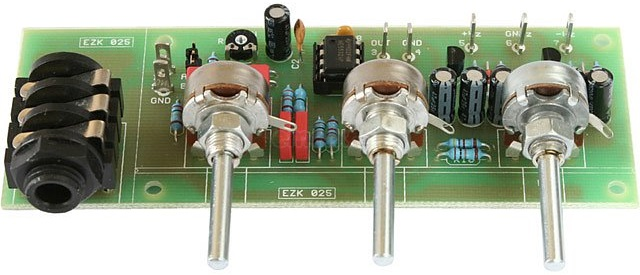
\includegraphics[]{zesilovac_foto.jpg}
    \caption{Fotografie zhotoveného modulu RMD3212SX}
\end{figure}

Jádrem korekčního zesilovače je klasický Baxandallův korektor, kterému je předřazen
jeden stupeň pro úpravu zisku zesilovače.
Potenciometrem $\text{P}_1$ se provádí regulace hloubek a pomocí $\text{P}_2$ se
regulují výšky.
Jumperem J1 volíme citlivost pro vstup LINE nebo pro mikrofon.
Základní nastavení citlivosti pro mikrofon je nutno provést trimrem $\text{R}_8$.
Regulace hlasitosti se prování potenciometrem $\text{P}_3$.
Korektor je opatřen symetrickým stabilizátorem napájecího napětí.

\begin{figure}[H]
    \centering
    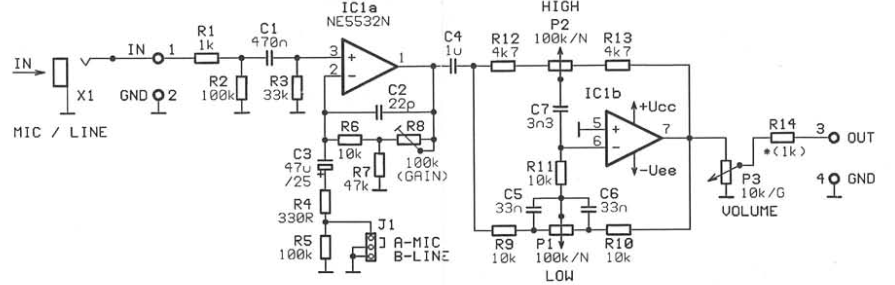
\includegraphics[width=0.8\textwidth]{zesilovac_schema.png}
    \caption{Schéma zapojení modulu RMD3212SX}
\end{figure}

\section{Úkoly měření}

\begin{enumerate}
    \item Během celého měření mějte citlivost vstupu nastavenou na LINE, tedy jumper v pozici B. Pokud nebude uvedeno jinak, trimr R8 mějte v poloze uprostřed. Také v přípravku ponechte zastrčený JACK konektor, který zabraňuje zkratování kontaktů ve vstupním konektoru. Pomocí přivedení signálu z generátoru a měření osciloskopem si zjistěte a zaznamenejte maximální vstupní napětí přípravku, kdy nedochází k limitaci na výstupu (na několika frekvencích ve slyšitelném pásmu a pro maximální nastavení potenciometru hlasitosti a maximální zdůraznění hloubek i výšek). Nezapomeňte aktivovat výstup generátoru pomocí stisku tlačítka Channel a volby Output On tlačítkem pod displejem. Jaká je maximální amplituda výstupního napětí, kdy ještě nedochází k limitaci? V dalších úkolech vždy nastavujte vhodné vstupní napětí tak, aby byla dostatečná rezerva před přebuzením zesilovače!
    \item Pomocí analyzátoru Bode 100 změřte frekvenční charakteristiky modulu a fáze přenosu (frekvence 20 Hz až 20 kHz, úroveň -27 dBm) pro nastavení potenciometrů hloubek a výšek v obou krajních polohách a uprostřed (celkem 9 kombinací). Potenciometr hlasitosti mějte nastavený na maximum.
    \item Pomocí analyzátoru Bode 100 změřte frekvenční charakteristiky modulu a fáze vstupní impedance (20 Hz – 20 kHz) a zjistěte, jak jsou závislé na nastavení potenciometrů.
    \item Zjistěte vliv trimru R8 na zesílení obvodu.
\end{enumerate}

\section{Seznam použitých přístrojů}

\begin{itemize}
    \item Modul monofonního korekčního zesilovače RMD3212SX
    \item Laboratorní napájecí zdroj Agilent E3630A
    \item Laboratorní digitální osciloskop Agilent DSO-X 2012A
    \item Laboratorní signálový generátor
    \item Obvodový analyzátor Bode 100
\end{itemize}

\section{Zpracování úkolů}

\subsection{Měření maximálního vstupního napětí přípravku (Úkol 1)}

V tomto úkolu jsme se věnovali zjištění maximální hodnoty vstupního napětí přípravku,
kdy nedochází k limitaci na výstupu na několika frekvencích ve slyšitelném pásmu
a pro maximální nastavení potenciometru hlasitosti a maximální zdůraznění hloubek i výšek.

Pro toto měření byl použit signálový generátor a osciloskop.
Generátor byl připojen na vstup přípravku a osciloskop na výstup.
Na generátoru jsme nejprve nastavili požadovaný kmitočet a poté jsme postupně zvyšovali
amplitudu signálu dokud jsme nepozorovali limitaci výstupního signálu přípravku na osciloskopu.
Napětí bylo poté změřeno osciloskopem a zaznamenáno do tabulky uvedené níže.
Měření bylo opakováno pro několik kmitočtů ve slyšitelném pásmu.

\begin{table}[H]
    \catcode`\-=12
    \centering
    \caption{Maximální vstupní napětí přípravku na několika kmitočtech}
    \begin{tabular}{lccccc}
        \toprule
        Kmitočet:    & 20\,Hz  & 100\,Hz & 1\,kHz  & 10\,kHz & 20\,kHz \\
        \cmidrule(rl){1-6}
        Max. napětí: & 1,95\,V & 2,23\,V & 8,75\,V & 2,43\,V & 2,07\,V \\
        \bottomrule
    \end{tabular}
\end{table}

%%%%%%%%%%%%%%%%%%%%%%%%%%%%%%%%%%%%%%%%%%%%%%%%%%%%%%%%%%%%%%%%%%%%%%%%%%%%%%%%
%\textbf{DOPLNIT POPIS POZOROVANÉHO JEVU}
%%%%%%%%%%%%%%%%%%%%%%%%%%%%%%%%%%%%%%%%%%%%%%%%%%%%%%%%%%%%%%%%%%%%%%%%%%%%%%%%
Z výsledků je patrné, že práh přebudení obvodu vstupním signálem je pro jednotlivé frekvence různý.

\subsection{Měření frekvenční charakteristiky modulu a fáze přenosu (Úkol 2)}

V tomto úkolu jsme pomocí analyzátoru Bode 100 měřili frekvenční charakteristiky
modulu a fáze přenosu pro několik různých nastavení potenciometrů hloubek, výšek a hlasitosti.

Analyzátor Bode 100 byl nejdříve v programu Bode Analyzer Suite nastaven na měření
frekvenčních charakteristik ve slyšitelném pásmu.
Poté bylo potřeba analyzátor před samotným měřením zkalibrovat.
Výsledné charakteristiky byly zobrazeny na obrazovce počítače a vloženy do protokolu
níže formou snímků obrazovky.

\begin{figure}[H]
    \centering
    \begin{subfigure}{0.49\textwidth}
        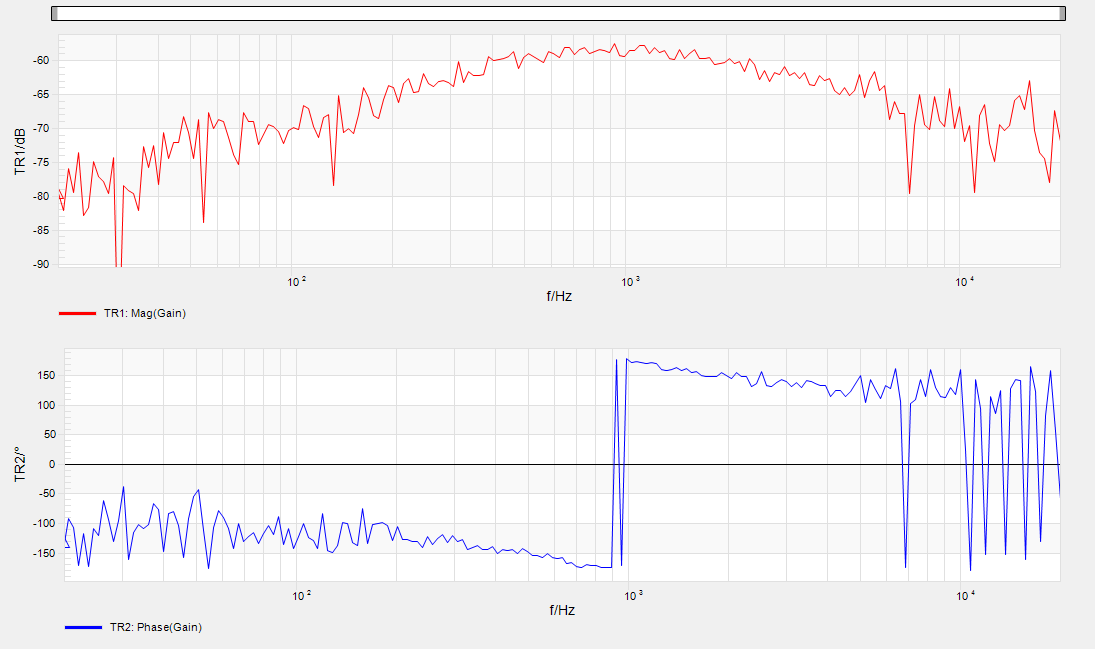
\includegraphics[width=\textwidth]{nkzt9_2_min_min_min.png}
        \caption{Minimální krajní poloha}
    \end{subfigure}
    \hfill
    \begin{subfigure}{0.49\textwidth}
        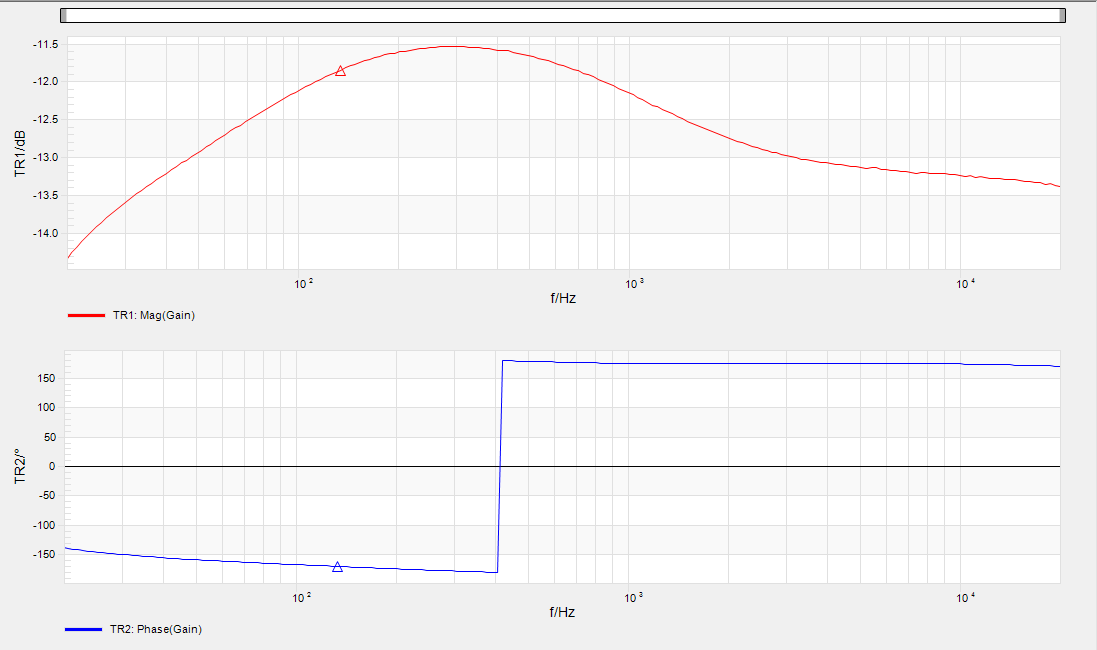
\includegraphics[width=\textwidth]{nkzt9_2_mid_mid_mid.png}
        \caption{Poloha uprostřed}
    \end{subfigure}

    \begin{subfigure}{0.49\textwidth}
        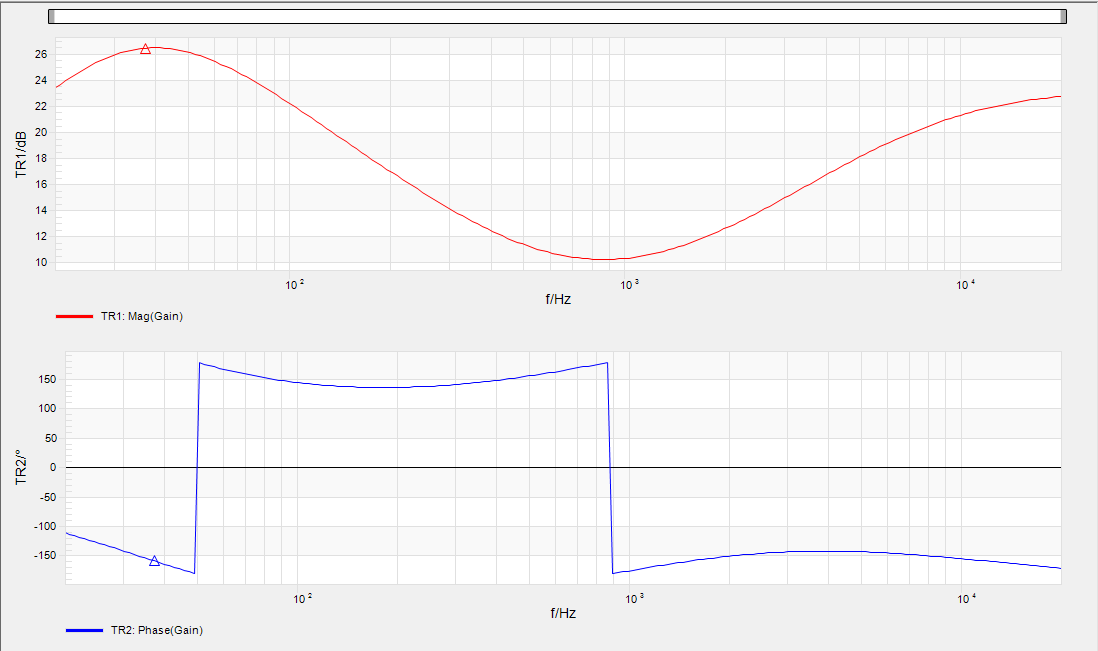
\includegraphics[width=\textwidth]{nkzt9_2_max_max_max.png}
        \caption{Maximální krajní poloha}
    \end{subfigure}
    \caption{Frekvenční charakteristiky modulu a fáze přenosu pro nastavení všech potenciometrů} 
\end{figure}

\begin{figure}[H]
    \centering
    \begin{subfigure}{0.49\textwidth}
        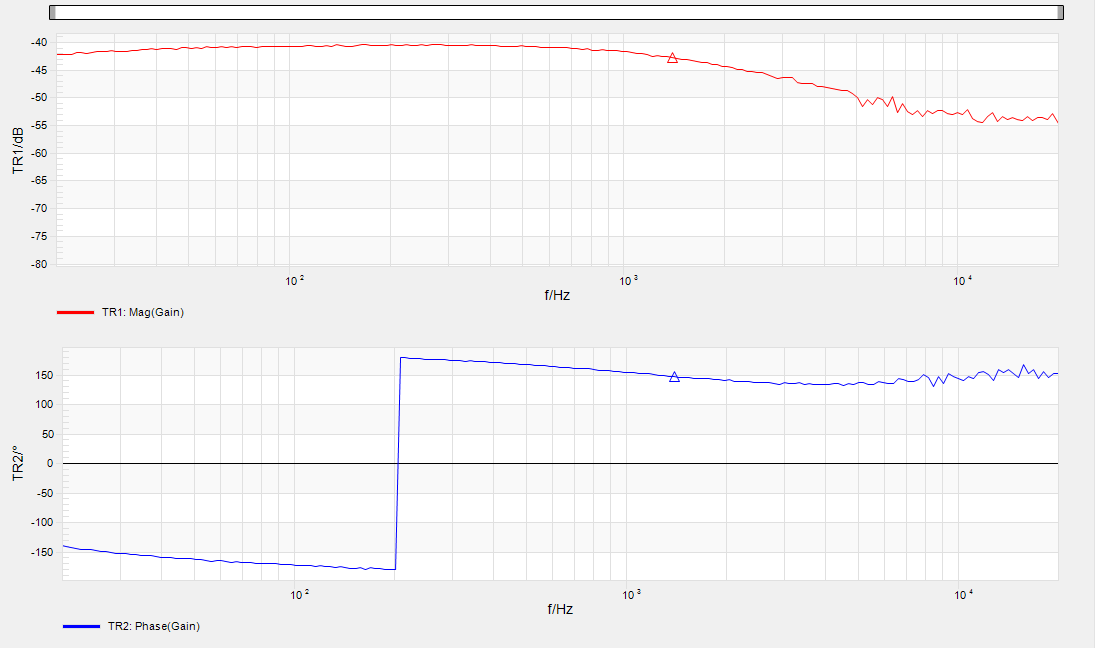
\includegraphics[width=\textwidth]{nkzt9_2_mid_min_min.png}
        \caption{Poloha uprostřed}
    \end{subfigure}
    \hfill
    \begin{subfigure}{0.49\textwidth}
        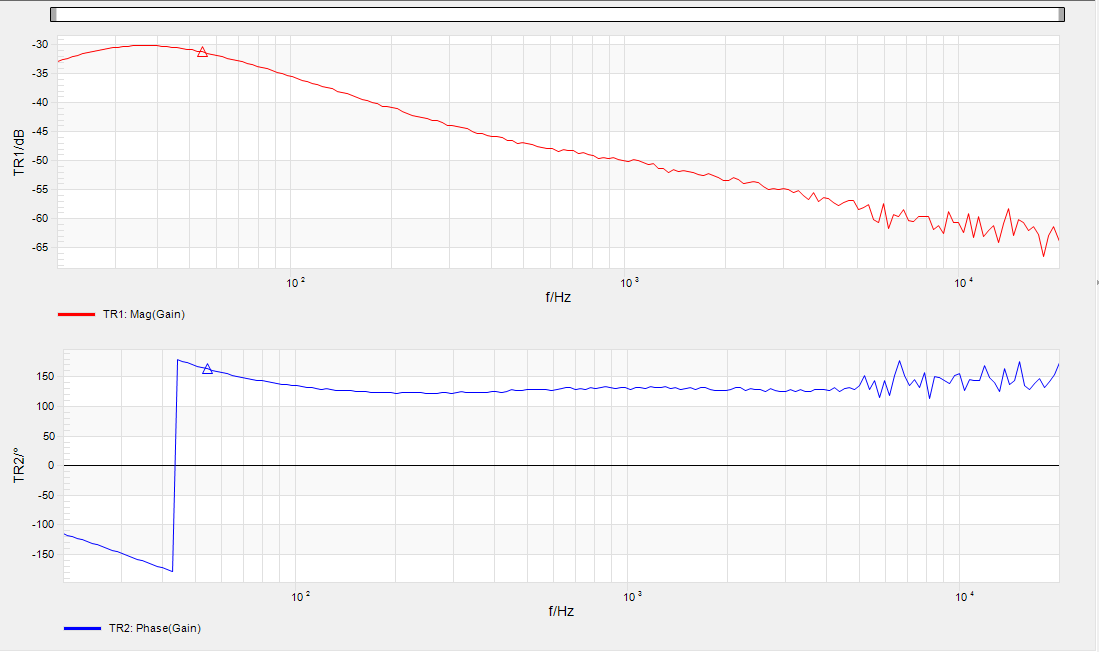
\includegraphics[width=\textwidth]{nkzt9_2_max_min_min.png}
        \caption{Minimální krajní poloha}
    \end{subfigure}
    \caption{Frekvenční charakteristiky modulu a fáze přenosu pro nastavení potenciometru hloubek} 
\end{figure}

\begin{figure}[H]
    \centering
    \begin{subfigure}{0.49\textwidth}
        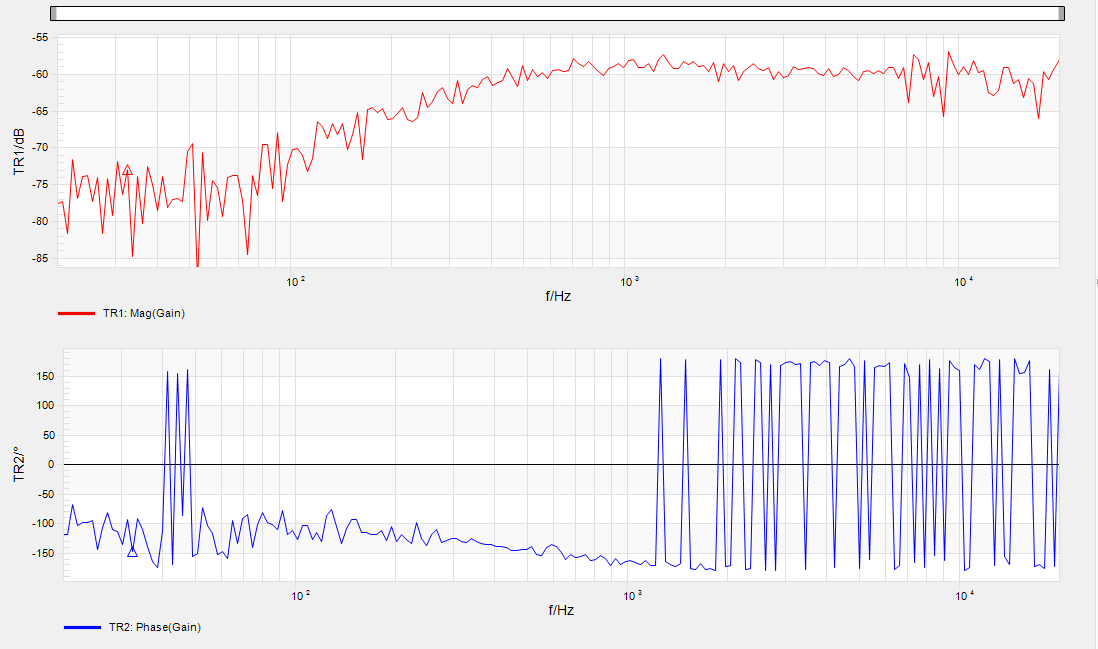
\includegraphics[width=\textwidth]{nkzt9_2_min_mid_min.png}
        \caption{Poloha uprostřed}
    \end{subfigure}
    \hfill
    \begin{subfigure}{0.49\textwidth}
        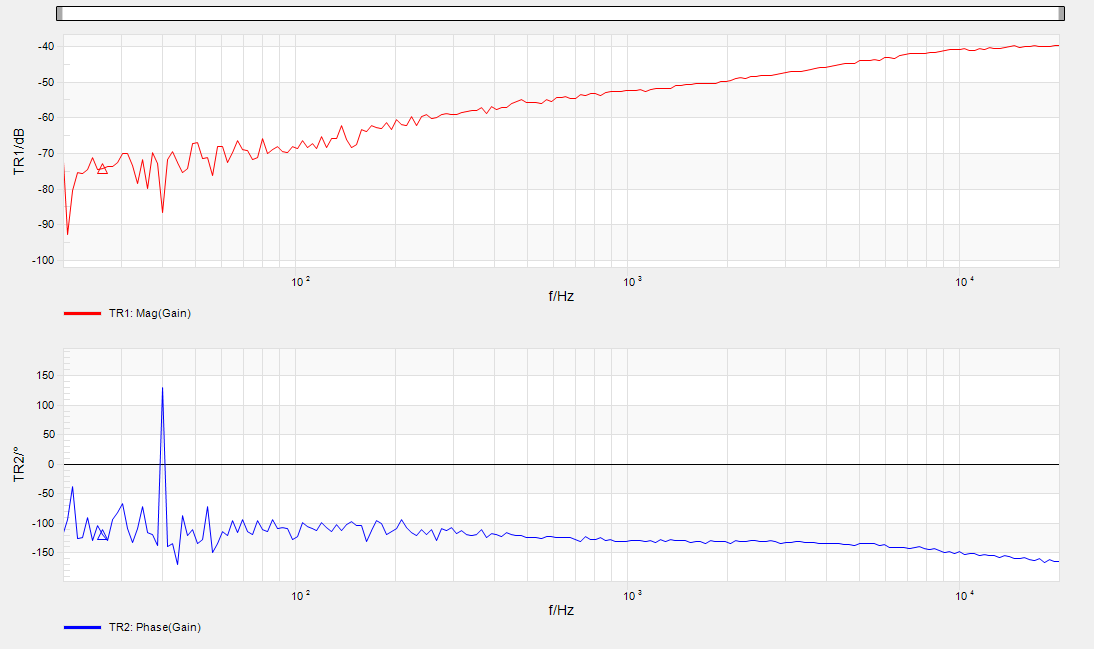
\includegraphics[width=\textwidth]{nkzt9_2_min_max_min.png}
        \caption{Minimální krajní poloha}
    \end{subfigure}
    \caption{Frekvenční charakteristiky modulu a fáze přenosu pro nastavení potenciometru výšek} 
\end{figure}

\begin{figure}[H]
    \centering
    \begin{subfigure}{0.49\textwidth}
        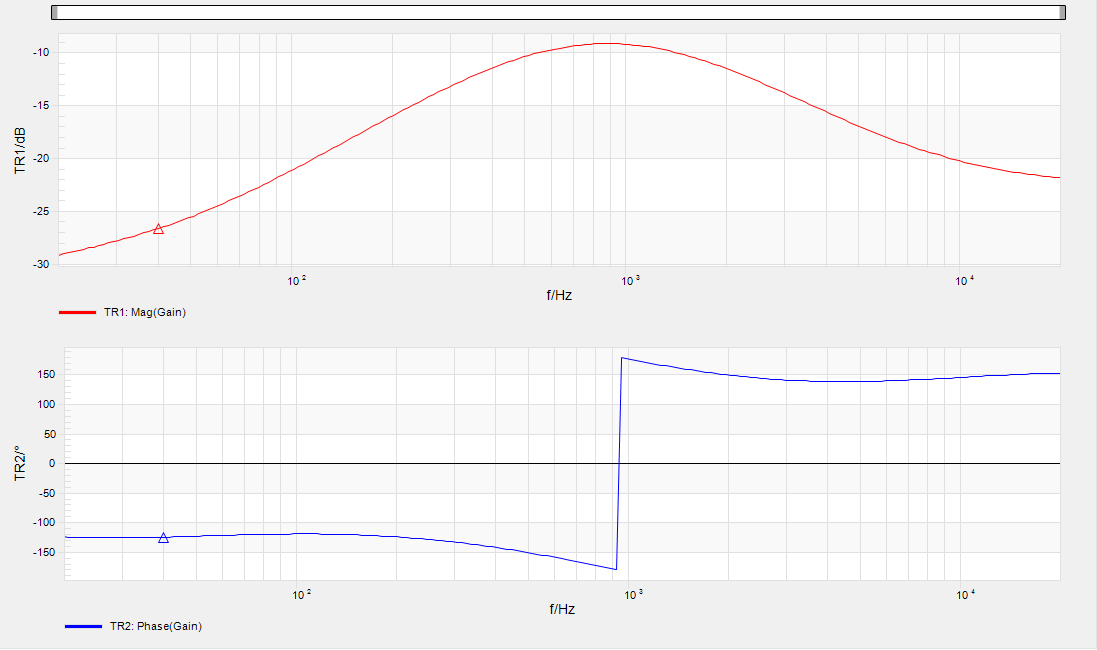
\includegraphics[width=\textwidth]{nkzt9_2_min_min_mid.png}
        \caption{Poloha uprostřed}
    \end{subfigure}
    \hfill
    \begin{subfigure}{0.49\textwidth}
        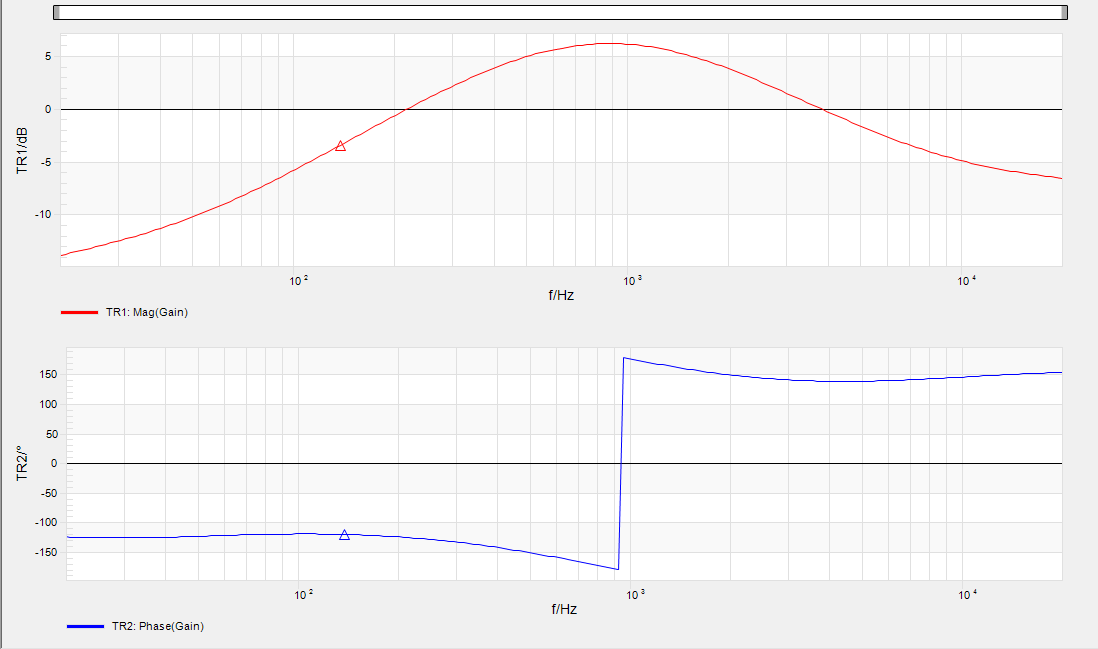
\includegraphics[width=\textwidth]{nkzt9_2_min_min_max.png}
        \caption{Minimální krajní poloha}
    \end{subfigure}
    \caption{Frekvenční charakteristiky modulu a fáze přenosu pro nastavení potenciometru hlasitosti} 
\end{figure}

\subsection{Měření frekvenční charakteristiky modulu a fáze vstupní impedance (Úkol 3)}

V tomto úkolu jsme opět pomocí analyzátoru Bode 100 měřili frekvenční charakteristiky
modulu a fáze impedance pro různé nastavení potenciometrů hloubek, výšek a hlasitosti.
Našim cílem bylo tentokrát zjistit závislost těchto charakteristik na nastavení potenciometrů.

Analyzátor Bode 100 byl nejdříve v programu Bode Analyzer Suite nastaven na měření
frekvenčních charakteristik impedance ve slyšitelném pásmu.
Poté bylo potřeba analyzátor před samotným měřením zkalibrovat.
Výsledné charakteristiky byly zobrazeny na obrazovce počítače a vloženy do protokolu
níže formou snímků obrazovky.

\begin{figure}[H]
    \centering
    \begin{subfigure}{0.49\textwidth}
        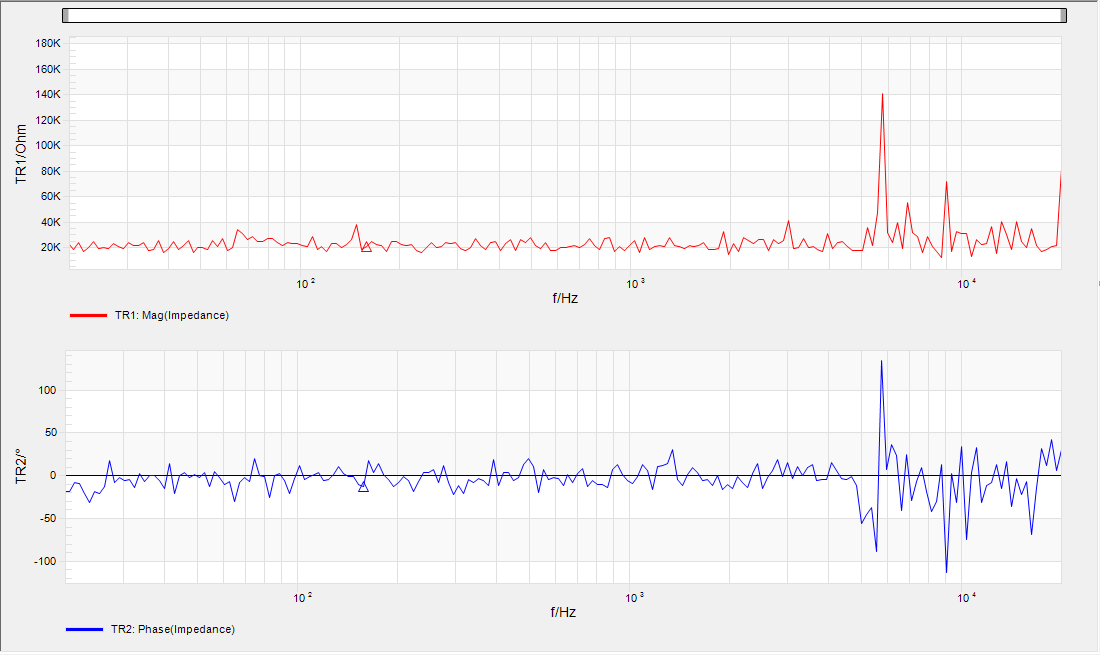
\includegraphics[width=\textwidth]{nkzt9_3_min_min_min.png}
        \caption{Minimální krajní poloha potenciometrů}
    \end{subfigure}
    \hfill
    \begin{subfigure}{0.49\textwidth}
        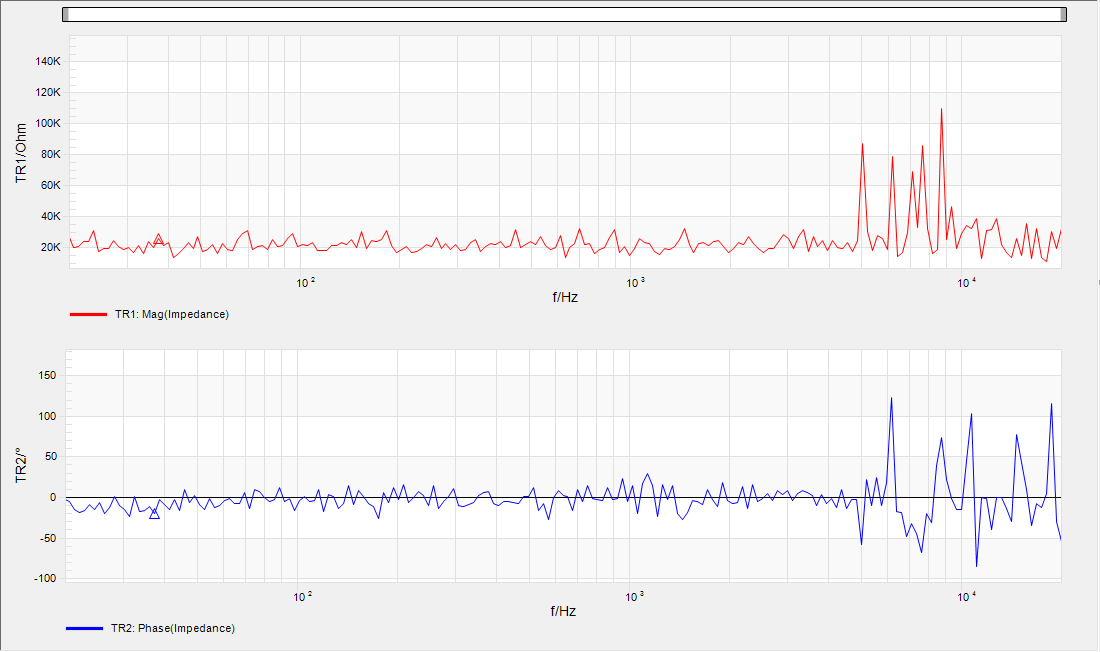
\includegraphics[width=\textwidth]{nkzt9_3_max_max_max.png}
        \caption{Maximální krajní poloha potenciometrů}
    \end{subfigure}
    \caption{Frekvenční charakteristiky modulu a fáze vstupní impedance} 
\end{figure}

%%%%%%%%%%%%%%%%%%%%%%%%%%%%%%%%%%%%%%%%%%%%%%%%%%%%%%%%%%%%%%%%%%%%%%%%%%%%%%%%
%\textbf{DOPLNIT POPIS POZOROVANÉHO JEVU}
%%%%%%%%%%%%%%%%%%%%%%%%%%%%%%%%%%%%%%%%%%%%%%%%%%%%%%%%%%%%%%%%%%%%%%%%%%%%%%%%
Na výsledných naměřených charakteristikách pozorujeme, že nastavení potenciometrů nemělo výrazný vliv.
Nemužeme to však říct s jistotou kvůli velkému šumu ve výsledných grafech, který je způsoben měřením velké hodnoty impedance oproti hodnotě 50 \(\Omega\)
% Něco dál? nevím...

\subsection{Měření vlivu trimru $\text{R}_8$ na zesílení (Úkol 4)}

V posledním úkolu jsme se věnovali zjištění vlivu nastavení polohy trimru $\text{R}_8$ na zesílení
výstupního signálu přípravku.

K tomuto měření byl opět použit generátor na vstupu obvodu a osciloskop na výstupu.
Na generátoru byl nastaven signál se sinusových průběhem o kmitočtu 1\,kHz.
Amplituda signálu byla volena tak, aby nedošlo k limitaci výstupního signálu přípravkem
dle hodnot tabulky v úkolu č.1.
Dále byly zhotoveny snímky obrazovky osciloskopu pro různá nastavení polohy trimru,
které byly do protokolu vloženy níže.

\begin{figure}[H]
    \centering
    \begin{subfigure}{0.49\textwidth}
        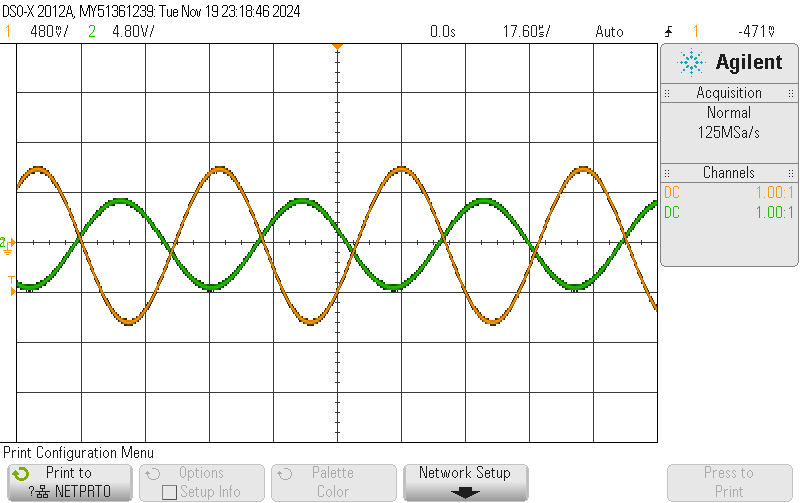
\includegraphics[width=\textwidth]{osc_min.png}
        \caption{Minimální krajní poloha}
    \end{subfigure}
    \hfill
    \begin{subfigure}{0.49\textwidth}
        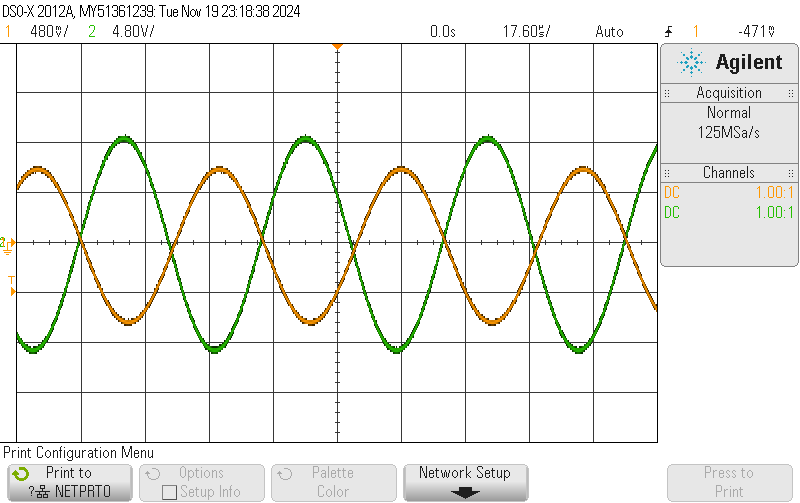
\includegraphics[width=\textwidth]{osc_mid.png}
        \caption{Poloha uprostřed}
    \end{subfigure}

    \begin{subfigure}{0.49\textwidth}
        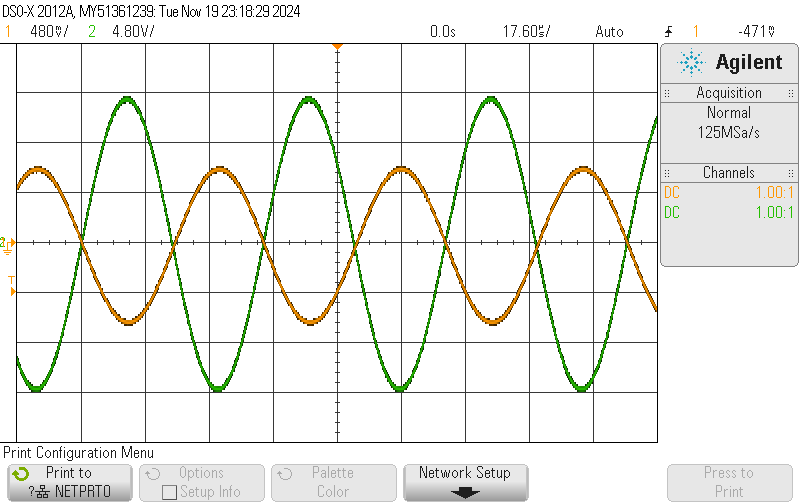
\includegraphics[width=\textwidth]{osc_max.png}
        \caption{Maximální krajní poloha}
    \end{subfigure}
    \caption{Snímky obrazovky osciloskopu pro různá nastavení trimru $\text{R}_8$} 
\end{figure}

%%%%%%%%%%%%%%%%%%%%%%%%%%%%%%%%%%%%%%%%%%%%%%%%%%%%%%%%%%%%%%%%%%%%%%%%%%%%%%%%
%\textbf{DOPLNIT POPIS POZOROVANÉHO JEVU}
%%%%%%%%%%%%%%%%%%%%%%%%%%%%%%%%%%%%%%%%%%%%%%%%%%%%%%%%%%%%%%%%%%%%%%%%%%%%%%%%

Pozorujeme, že došlo k zesílení signálu v závislosti na poloze trimru. % Víc nevim...

\section{Závěr}
V úloze proběhlo měření sestaveného obvodu korekčního zesilovače, který je postavem na operačním zesilovači NE5532. Jedná se o nízkošumový OZ a to ho činní ideálním pro takovéto aplikace v oblasti audiotechniky. 

%%%%%%%%%%%%%%%%%%%%%%%%%%%%%%%%%%%%%%%%%%%%%%%%%%%%%%%%%%%%%%%%%%%%%%%%%%%%%%%%
%\textbf{DOPLNIT ZÁVĚR}
%%%%%%%%%%%%%%%%%%%%%%%%%%%%%%%%%%%%%%%%%%%%%%%%%%%%%%%%%%%%%%%%%%%%%%%%%%%%%%%%
% Více méně to samé jako v popisech pozorovaných jevů

\end{document}
